\documentclass[a4paper, usenatbib, 12pt]{article}
\usepackage{subfig}
\usepackage{float}
\usepackage{wrapfig}
\usepackage{graphicx}
\usepackage{amsmath}
\usepackage{amssymb}
\usepackage{booktabs}
\usepackage{cite}
\usepackage[icelandic,spanish,english]{babel}
\usepackage[T1]{fontenc}
\usepackage[utf8]{inputenc}
\usepackage[top=3.5cm, bottom=2.5cm, left=3.5cm,right=3.5cm]{geometry} 

%----------------------New commands -------------------

\newcommand{\tol}{Tololo 1214-277}
\newcommand{\lya}{Ly$\alpha$}
\newcommand{\hb}{H$\beta$}
\newcommand{\ha}{H$\alpha$}
\newcommand{\oiii}{[OIII]}
\newcommand{\oii}{[OII]}
\newcommand{\nii}{[NII]}
\newcommand{\esca}{erg cm$^{-2}$ s$^{-1}$ \AA$^{-1}$}
\newcommand{\esc}{erg cm$^{-2}$ s$^{-1}$}
\newcommand{\es}{erg s$^{-1}$}
\newcommand{\esa}{erg s$^{-1}$}
\newcommand{\kms}{km s$^{-1}$}
\newcommand{\apj}{ApJ}  
\newcommand{\jcap}{JCAP}  
\newcommand{\apjs}{ApJS}  
\newcommand{\apjl}{ApJL}  
\newcommand{\aj}{AJ}  
\newcommand{\mnras}{MNRAS}  
\newcommand{\mnrassub}{MNRAS accepted}  
\newcommand{\aap}{A\&A}  
\newcommand{\aaps}{A\&AS}  
\newcommand{\araa}{ARA\&A}  
\newcommand{\nat}{Nature}  
\newcommand{\physrep}{PhR}
\newcommand{\pasp}{PASP}    
\newcommand{\pasj}{PASJ}    
\def\simgt{\lower.5ex\hbox{\gtsima}}
\def\simlt{\lower.5ex\hbox{\ltsima}}
%------------------------------------------------------

\begin{document}
\pagestyle{empty}
\noindent
\textbf{Þú ert jörðin}
\\
\\
JEFR$^{1}$, MCRG$^1$, JNGC$^2$, MD$^3$
\\
\\
\scriptsize
{$^1$ Bogota
\\
$^2$ Tucson
\\
$^3$ Oslo
\normalsize
\\
\\
\textbf{
  Star-forming Compact Dwarf Galaxies (CDGs) resemble the expected
  pristine conditions of the first galaxies in the Universe.    
Before the observational detection of the first galaxies becomes
reality, CDGs are the best systems to test our ideas on primordial
galaxy formation and evolution.    
Here we report on one of such CDGs, \tol, which presents
features in its Lyman-$\alpha$ emission thad had evaded theoretical
interpretation so far. 
We show that these special features, a symmetric triple peaked
emission line, can be explained by gas bulk rotation.  
We find that the Lyman-$\alpha$ emission region in \tol\ should
have a rotational velocity of $V_{r}=300$ km s$^{-1}$ and a neutral
Hydrogen column density of $\log N_{HI} / \mathrm{atoms\ cm}^{-2} =
  20.5$.   
Using archival observational information about \tol\ we find that the
diameter for that emission region diameter should be in the range of
$110$ pc $<D<$ $340$ pc and its total dynamical mass   should be
between $2.1\times 10^{9}$M$_{\odot}$ $<M_D<$  $6.6\times
10^{9}$M$_{\odot}$.  
This dynamical mass is at least $16\pm 9$ times
larger than the neutral mass hydrogen.
We argue that a possibility to explain the excess in
dynamical mass is the presence of a super-massive black hole. }  



The first generation of galaxies trace our cosmic origins. 
They were the first steps in the evolution of galaxies such as the Milky
Way. 
In the standard Big Bang cosmology the only elements that were
created in the nucleosynthesis process were Hydrogen, Helium and
Lithium. 
Heavier elemets must have been created in stellar evolution process. 
Therefore, we expect the first generation of
galaxies to be metal free and rich in Hydrogen. 
This kind of primordial galaxies have not been detected yet. 
However, dwarf star forming galaxies with a low metallicity content
are seen as templates to understand the early galaxy evolution process. 

Almost fifty years ago \cite{PartridgePeebles} it was realized that
young galaxies could be detected through a strong Lyman-$\alpha$ line
emission.  
This theoretical prediction was only confirmed thirty year later on
distant relatively young, not primordial, galaxies.
Currently Lyman Alpha Emitting (LAE) galaxies are commonly targetted
in surveys. 
The presence of the Ly-$\alpha$ emission line provides confirmation of
the distance of a galaxy while provides clues about the stellar
population and inter-stellar medium conditions regulating the
Ly-$\alpha$ emission. 

The Ly-$\alpha$ emission line is not exclusive of distant galaxies. 
Any galaxy with low dust content and ongoing star formation has the
right conditions to show this line.  
There are, for instance,  local Universe surveys that target
Ly-$\alpha$ emission in nearby dwarf star forming galaxies. 
\cite{LARS}. 
The study of nearby LAE samples has allowd the study of other
indicators that might be more difficult to obtain for distant galaxies
such as morphology, dust attenuation, neutral hydrogen contents and
ionization state.  

However, the physical interpratation of Ly-$\alpha$ observations is
not straightforward. 
This is due to the resonant nature of the Ly-$\alpha$ line. 
A Ly-$\alpha$ photon follows a difussion-like process before escaping
the galaxy or being absorbed by dust. 
The resulting line profile becomes sensitive to the dynamical, chemical
and thermal conditions in the interstellar medium. 
There are very few analytical tools available to interpret the
Ly-$\alpha$ line.
They are applicable only in very few cases of highly symmetrical
conditions, which are hardly met in real astrophysical systems.

For these reasons the interpretation of Ly-$\alpha$ observations
require state-of-the-art montecarlo radiative transfer simulations.   
Recent advances in these computational models
\cite{GaravitoCamargo2014} have shown that galaxy rotation imprints an
effect on the Lyman-$\alpha$ line.
The most important consequence of rotation is that even for a
spherical gas distribution, the line morphology now depends on the
viewing angle respect to the rotation axis.  
For a line of sight perpendicular to the rotation axis the intensity
and the line center and the line width increase with rotational
velocity. 
When the rotational velocity is close to the half-line width of the
static line the line becomes single peaked, as it is observed in
\tol, a unique feature that other theoretical models find
difficult to reproduce without invoking complex gas distributions.

\tol\ is a compact star forming dwarf galaxies (CDGs) that presents a
strong Ly-$\alpha$ emission \cite{Thuan97} with two features that had
so far evaded a natural physical interpratation.
First, it has symmetric profile  without any systemic displacement
from the expected line-center. 
Second, it shows a triple peak, while the most common observational
feature corresponds either to a single or asymetric double peak. 
We have attempted an interpretation of the Ly-$\alpha$ line in
\tol\ by including the effect of gas bulk rotation.
We find that this model provides a satisfactory explanation of \tol's
puzzling features. 


Figure 1. summarizes our findings.
Dots represent the observational data for \tol with the
overplot from our best fit model from the full radiative transfer
simulation.   
The parameters for the best fit are
$v_{max}=300$\kms, $\tau=1\times10^7$, $T=1.5\times 10^{4}$K.
The optical depth and temperature can be translated into a column
density of $\log N_{HI} / \mathrm{atoms\ cm}^{-2} =
  20.5$.   
Our model is also able to constrain the angle
between the rotation axis and the observational line-of-sight to $\theta=65^{\circ}\pm$.
To determine the uncertainties we perform a Markov Chain Monte
Carlo calculation using an approximate analytical solution for the
Ly-$\alpha$ spectrum including rotational effects.


Radio surveys of the 21cm line have put an upper limit to the neutral
hydrogen mass in \tol of $M<2.65\times 10^{8}$ M$_{\odot}$. 
Together with our velocity and column density results, under the
assumption of spherical symmetry, we can constrain the total dynamical
mass of the HI region to be in the range $2.1\times 10^{9}$M$_{\odot}$
$<M_D<$  $6.6\times 10^{9}$M$_{\odot}$ and the diameter of HI region
should have a diameter of $0.11 < D/\mathrm{kpc}<0.34$. 
This makes the
dynamical mass  at least $7$ to $25$ times larger than the H$I$ mass. 

We consider three possibilities to explain the dynamical 
mass: stars, dark matter and a supermassive black hole. 
The stellar mass can be constrained by measurements of the 
stellar continuum, this can only represent $xx$M$_{\odot}$ of the total
contribution. 
Considering a standard dark matter halo, it can only constributio to
$xx$ M$_{\odot}$ in the region of interest. 
A super massive black hole remains an open  possibility. 
Recent observations of ultra-compact dwarf galaxies
\cite{Seth2014} have confirmed the presence of super-massive black
holes containing $15\%$ of the total object mass, suggesting that
there is a large population of undetected black holes in dwarf
galaxies.  

A future observational test of this possibility in \tol\ would require
integral field unit measurements spatially resolving its spatial
extent. 
\tol\ spans a region of $\approx 4$ arcminutes. 
An instrument such as the Multi Unit Spectroscopic Explorer with its
nominal $0.2$ arcseconds spatial sampling over a $1.0$ arcminute field
in wide-field mode could provide a detailed mapping of different
ionization lines to infer a kinematic map.

Why is triple peaked emission not common in  Lyman-alpha emitting
gaalaxies?   
The ubiuquity of galaxy outflows overimposed to the rotation
transforms the line into the common double or single peaked
line.
Therefore, the absence of HI outflows in \tol\ is another special
feature that permitted a symmetric triple peaked lya line to emerge. 

The implications of our finding for the study of LAEs, including the
first generation of galaxies are manifold. 
First of all, it demonstrated the importance of including rotation as
theoretical feature to interpret observed spectra. 
Secondly, it provides a motivation to explore under what conditions
rotation dominated dynamics are expected in comparison with outflow
dominated dynamics. 
Finally, if the hypothesis of a supermassive black
hole in \tol\ proves to be consistend with future observational
kinematic maps, it would provide a new information to test and probe
theories on the coevolution of galaxies and black holes in the first
generation of galaxies. 



\begin{figure}
\begin{center}
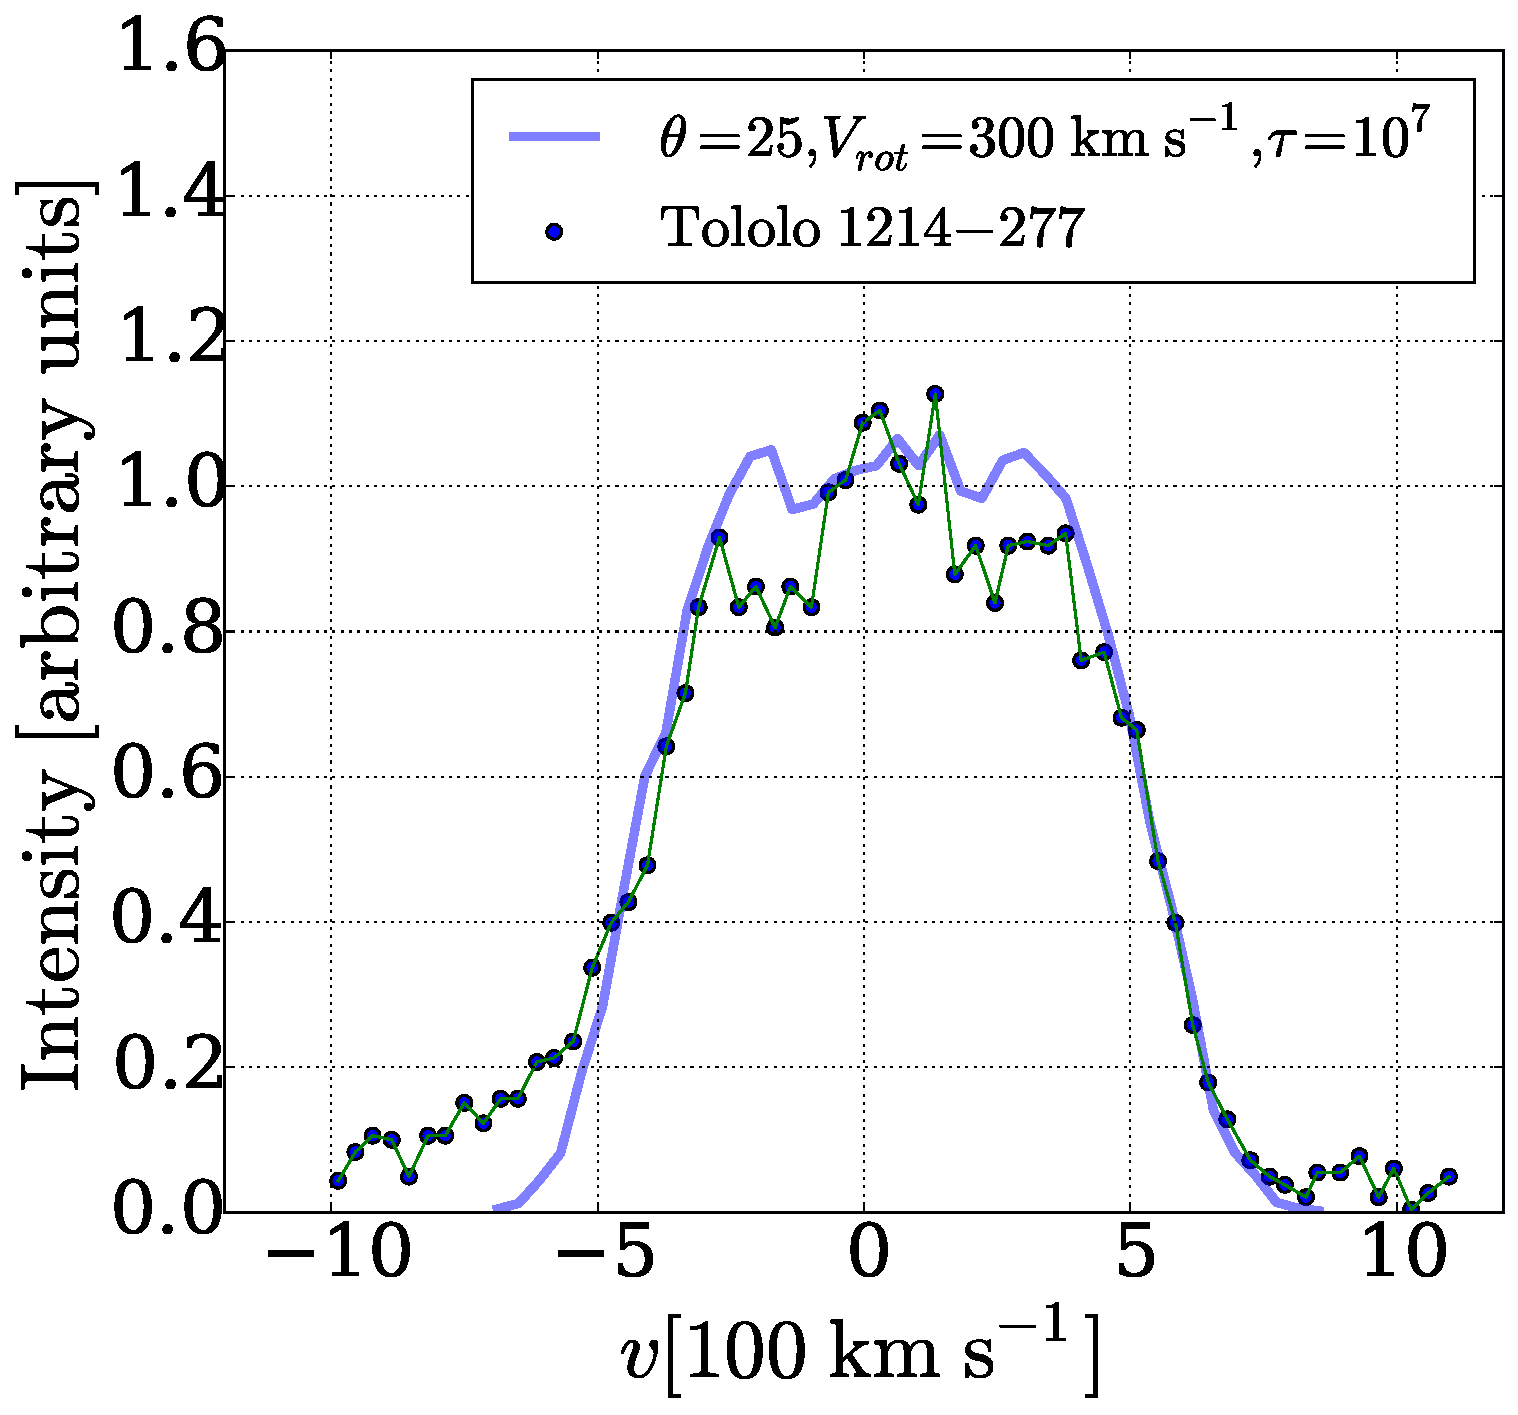
\includegraphics[width=0.8\textwidth]{tolfit.pdf}
\caption{{\bf Symmetric triple peaked Ly-$\alpha$ emission of \tol.}
  Dots correspond to the observational data. The line shows the result
of our best model from a full radiative transfer simulation. The best
parameters correspond to a rotational velocity of $300$km s$^{-1}$,
neutral Hydrogen optical depth of $10^{7}$ and a viewing angle of
$65^{\circ}$ measured from the rotation axis.} 
\end{center}
\end{figure}

\bibliography{references}{}
\bibliographystyle{plain}

\newpage 

\section*{\tol\ characteristics}


\begin{table}
\begin{center}
\begin{tabular}{lc}
$\alpha$(2000)$^{a}$ & 12h17min17.1s\\
$\delta$(2000)$^{b}$ & -28d02m32s\\
$l$, $b$ (deg) & 294, 34\\
$m_V$ & 17.5\\
  M$_V$ & -17.6\\ 
$v$(km s$^{-1}$) & 7795\\
Ly-$\alpha$ (erg cm$^{-2}$ s$^{-1}$ \AA$^{-1}$)& $8.1\times 10^{-14}$ \\
Ly-$\alpha$ EW & $70$\AA\\
H$\beta$ (erg cm$^{-2}$ s$^{-1}$ \AA$^{-1}$) & $1.62\times 10^{-14}$ \\
$21$cm (Jy km s$^{-1}$)& $<0.10$ \\
\end{tabular}
\end{center}
\caption{Basic observational characteristics of TOL1214-277
  \cite{Thuan97}\\} 
\end{table}



\tol receeding velocity is $7785\pm 50$km s$^{-1}$, which translates
into a distance of $106.6$ Mpc (Hubble constant 73 Mpc km$^{-1}$
s$^{1}$)
Its metallicity is $\sim Z_{\odot}/24$ \cite{Izotov04} as derived from optical
spectroscopy. 


The observed flux for the Lyman alpha line is $\sim
8.1\times 10^{-14}$ erg cm$^{-2}$ s$^{-1}$ \cite{Thuan97}
and a Equivalent Width of $70$\AA and its H$\beta$ flux is 
$1.62\times 10^{-14}$ erg cm$^{-2}$ s$^{-1}$ \AA${-1}$
\cite{Izotov04} which gives a Ly$\alpha$/H$\beta$ flux ratio of
4.9$\pm$0.1. The Ly-$\alpha$ flux values correspond to luminosities of
$L_{Ly\alpha}=2.2\times 10^{42}$ erg s$^{-1}$ over a $20$\AA
bandwidth, which in turns translates  into a star formation rate of
$2.0$ M$_{\odot}$ yr$^{-1}$ using a standard conversion factor between
luminosity and star formation rate of $9.1\times 10^{-43}$
$L_{Ly\alpha}$ M$_{\odot}$ yr$^{-1}$. 
The absolute magnitude in the $V$ band translates into a luminosity of
$8.9\times 10^{8}$ L$_{\odot}$.
% using http://tomdwelly.com/tools_fluxtolum.php
Comparing this ratio with the theoretical expectation from case B
recombination of $23.3$ \cite{Hummer1987} one can estimate an escape
fraction of $20$\% for Ly$\alpha$ radiation.

The optical emission  comes from a   region with approximate diameter
?? \cite{Fricke01}. 

\section*{MCMC constraints}

\section*{Physical Interpretation}

Interpretation by \cite{mashesse03}.

There is an upper limit for the  
integrated flux of $<0.10$ Jy km s$^{-1}$, which translates into a
upper limit for the HI mass of $M<2.65\times 10^{8}$ M$_{\odot}$
\cite{pustilnikmartin07}. 
From the optical depth of $10^7$ and the non-detection in the HI line,
we have an upper limit for the size where the Lya emission comes of
$D<0.34$kpc. 

 For an homogeneous sphere the HI optical depth from its can be
 written as $\tau = \sigma_0 n D/2$, where $\sigma_0=5.898\times
10^{-14}$cm$^{-2}$ is the Lyman$\alpha$  optical depth at the 
line's center, $n$ is the number density and $D$ is the sphere's
diameter. 
From this we can impose additional constrains on $D$ from the tipical
values of the Hydrogen number density and our constrain on
$\tau=10^{7}$.  Using a range of $1<n/\mathrm{atoms/cm}^{-3} <
10^{-3}$. This gives us a range of $0.11 < D/\mathrm{kpc}<100$. 
Together from the total HI mass we have thus that the HI region should
have a diameter of $0.11 < D/\mathrm{kpc}<0.34$.



This can be rewritten in terms of the gas' temperature $T$ and column
density $N_{H}$as $\tau = 3.31 \times 10^{-14} (10^{4}\mathrm{K}/T)^{1/2}
(N_{H}/\mathrm{atoms\ cm}^{-2})$.  

This allows us to approximate the total hydrogen mass as
\begin{equation}
M_{H} = m_{H}  N_{H} D^{2} = 226\times \tau  \left(\frac{T}{10^4
  \mathrm{K}}\right)^{1/2}\left(\frac{D}{\mathrm{kpc}}\right)^2M_{\odot}
\end{equation}





On the other hand, we have an estimate for the dynamical mass from the
galaxy size $D$ and its rotational velocity $V$:



\begin{equation}
M_{T} = \frac{V^{2}D}{G} = 2.16\times10^{5}
\left(\frac{V}{\mathrm{km\ s}^{-1}}\right)^2\left(\frac{D}{\mathrm{kpc}}\right) M_{\odot}
\end{equation}


From this limit and the rotational velocity of $300$ km/s and the
limit in the size $D$ we have limits of for the dynamical mass of
$2.1\times 10^{9}$M$_{\odot}$ $<M_D<$  $6.6\times 10^{9}$M$_{\odot}$.
which is at least $7$ to $25$ times larger than the H$I$ mass. The
mass to luminosity ratio is in turn between $2$ to $7$ times
$L_{\odot}/M_{\odot}$ considering the total luminosity in the $V$
band. 


\section*{Joint Effect of Rotation and Outflow}

The almost complete absence of outflows is a central requirement for
reproducing the lyman alpha line in \tol. In this section we present
some results on the exploration of the presence of outflows join with
the bulk rotation. We defer a detailed exploration of this effects for
another publication. 

Figure XX shows the results of four different models. a) pure rotation
($V_{\rm rot}=100$ km s$^{-1}$), b) pure outflow ($V_{\rm out}=100$ km
s$^{-1}$), c) mixed outflow with rotation ($V_{\rm rot}=100$ km s$^{-1}$)($V_{\rm rot}=25$ km s$^{-1}$).



\end{document}

%% interpretation

